%%%%%%%%%%%%%%%%%%%%%%%%%%
\chapter{Experimental results}
\label{chap::EXPERIMENTAL RESULTS}
%%%%%%%%%%%%%%%%%%%%%%%%%%

\baselineskip=26pt

\section{Experiments on Regular Testcases for \cite{Ma08} and \cite{PH10}}
\label{sec::EXPERIMENTS ON REGULAR TESTCASES}
\begin{figure}[htb]
{
  \centering
  \scriptsize
   TABLE I: TESTCASE STATISTICS OF TWO DATA SETS
   \centerline{\includegraphics[width=10cm]{Fig/table_1.pdf}}
   %\centerline{\psfig{figure=Fig/table_1.eps, width=10cm}}

  \label{fig::table1}
}
\end{figure}

\begin{figure*}[htb]
  \centering
  \scriptsize
   TABLE II: COMPARISON BETWEEN \cite{Ma08} AND \cite{PH10} ON TWO DATA SETS
    \centerline{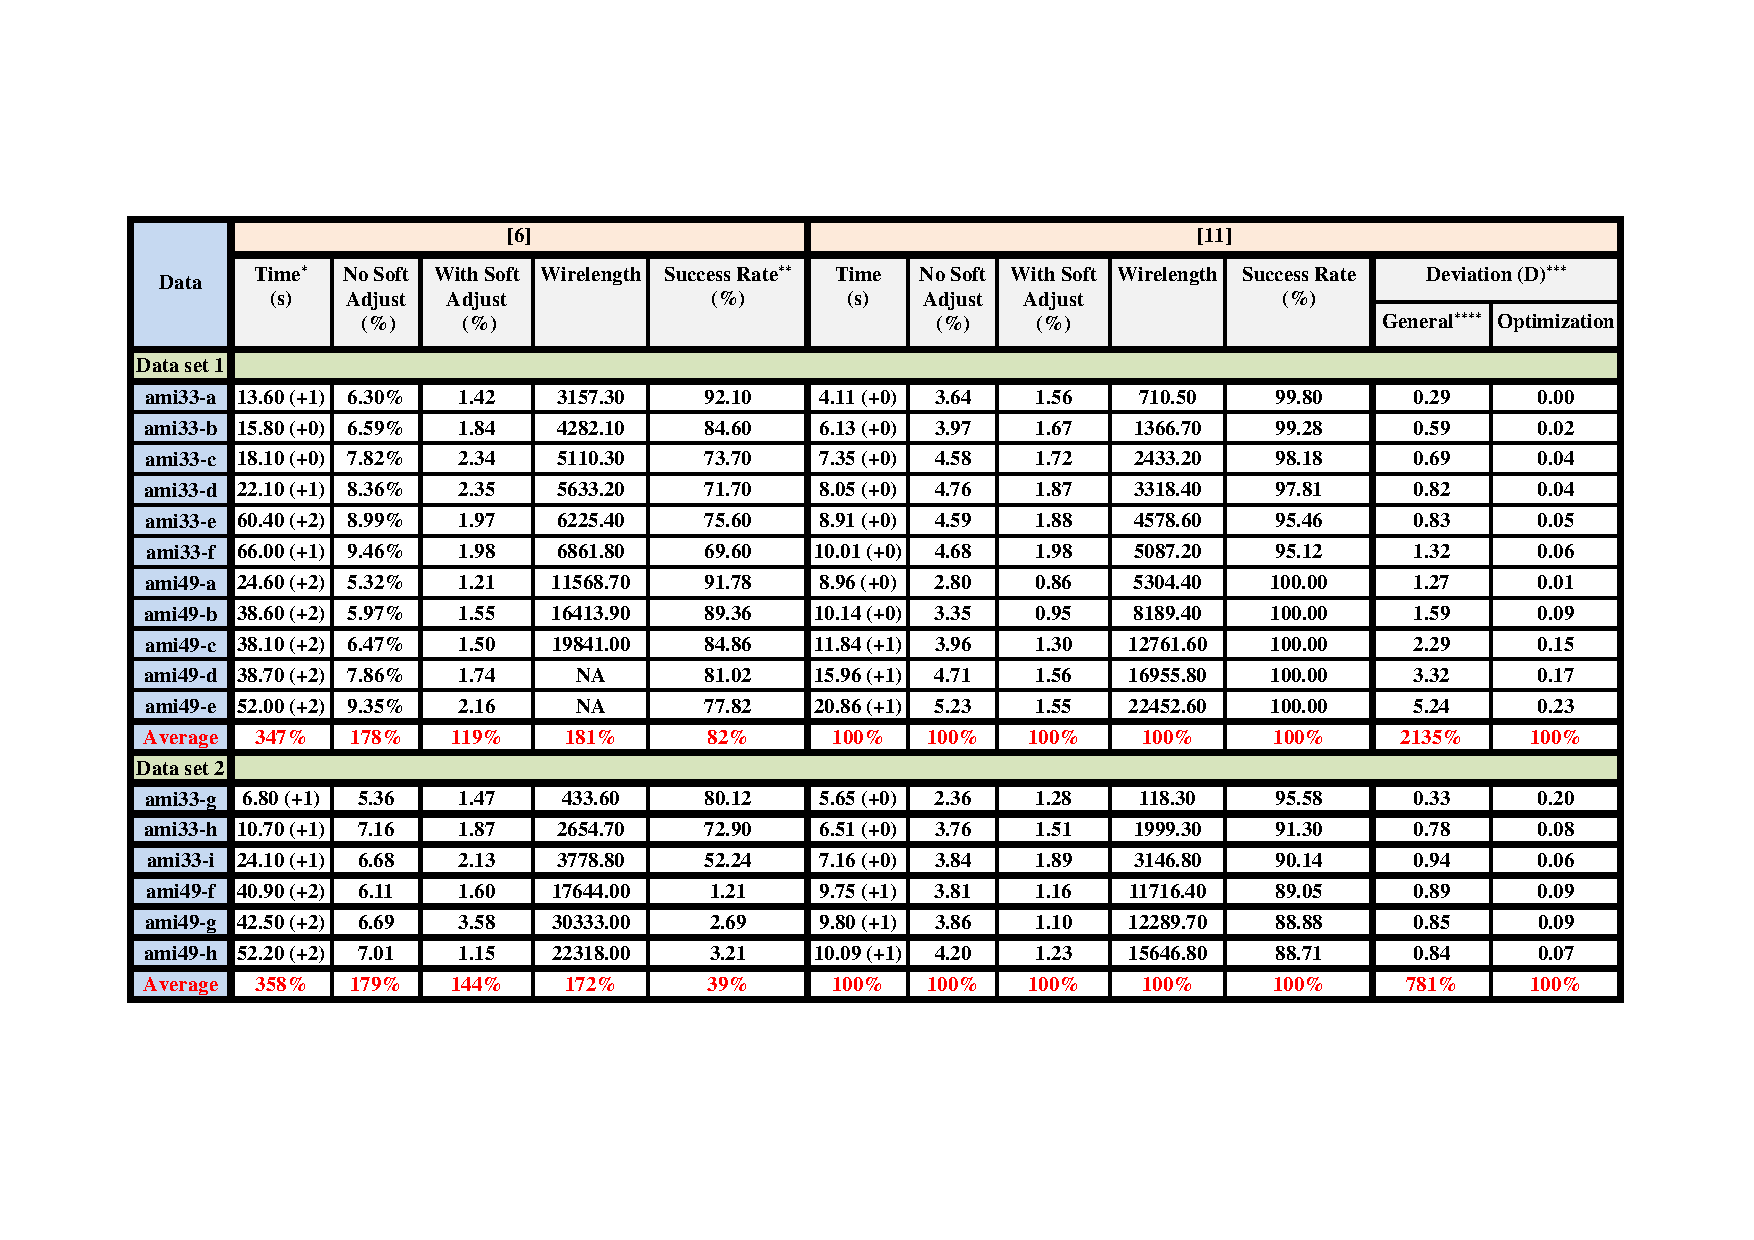
\includegraphics[width=17cm]{Fig/Table_2.pdf}}
    %\centerline{\psfig{figure=Fig/Table_2.eps, width=17cm}}\\
   $^*$Figures inside brackets represent the run time for soft module adjustment.\\
   $^{**}$The percentage of the floorplan generated by all iterations of the SA in which all the buses are feasible.\\
   $^{****}$The deviation (D) is obtained from total deviations at each load divided by total number of loads.\\
   $^{***}$The deviation at each load is estimated by total number of turning nodes from the driver to the load divided by total number of loads.
  \label{fig::TABLE_II}
\end{figure*}

In this section, we perform the experiments on the algorithm which
is published on GLSVLSI 2010 with the state-of-the-art bus-driven
floorplanner \cite{Ma08} which is published on ASPDAC 2008.
We implemented our bus-pin-aware bus-driven floorplanner in C
language on a 1.86-GHz Linux machine with 2GB memory. All
testcases are run by both our floorplanner and the
bus-driven floorplanner \cite{Ma08} on the same
machine. For fair comparison, each floorplanner runs ten times for
each testcase and the average is reported. Since the impact of the bus pin
is not considered in \cite{Ma08},
the bus pin of each module is not defined in the data set 1.
Therefore, we modify those testcases and assign the initial position
of each bus pin randomly.

In addition to perform experiments on data set 1 used in \cite{Ma08},
we also create data set 2 by modifying some testcases in data set 1 to
demonstrate the excellent routability of our algorithm. In data set
2, the bus width of each bus is wider than data set 1, i.e., it is more
difficult to obtain a feasible solution.
In each testcase, the first module of each bus is treated as the driver.
The details of all testcases are shown in Table I.

The first experiment is performed on data set 1, and the comparison results
are shown in Table II. As for the experiments about the
deviation of each module, for fair comparison, we only list the
average deviation (D) in the rightmost two columns for estimated and
optimized bus routing results from our floorplanner because
\cite{Ma08} does not consider the impact of the bus pins.
In this paper, we consider the diagonal connection
between two modules, it makes the bus shape more flexible, and the
size of the solution space is increased such that a better solution
can be obtained. Compared with \cite{Ma08}, the experimental
results show that our algorithm performs better in runtime by
3.47$\times$, success rate by 1.22$\times$, and reduced the
deadspace by 1.19$\times$. We also develop an algorithm to
reduce the wirelength, the experimental results show that our algorithm
performs better in wirelength by 1.81$\times$. By considering the
accumulated deviation during determining the position and
orientation of each bus pin, it can obtain better deviation at each load.
Experimental results show that the optimized deviation achieves 21.35$\times$
better than the estimated bus routing solution on average.
In our platform, \cite{Ma08}
does not generate a feasible final solution in ami49-d
and ami49-e, these testcases are ignored in wirelength
comparison. In other testcases, \cite{Ma08} fails to generate a
feasible final solution in some iterations of the ten annealing
processes, these iterations are also ignored in wirelength
comparison.

The experimental results of data set 2 are also shown in Table II.
Compared with \cite{Ma08}, the experimental results show that our
algorithm performs better in runtime by 3.58$\times$, success rate
by 2.56$\times$, and reduced the deadspace by 1.44$\times$. In
terms of wirelength, our algorithm performs better by 1.72$\times$.
With deviation optimization, the deviation achieves 7.81$\times$ better
than the estimated ones on average.
For ami49-f, ami49-g, and ami49-h, \cite{Ma08} could
not generate the feasible solution effectively. However, our
floorplanner still holds high solution quality in all aspects.
Some packing results are shown in Figure~\ref{fig::packing_result1}.

\begin{figure}[htb]
  \centering
  \centerline{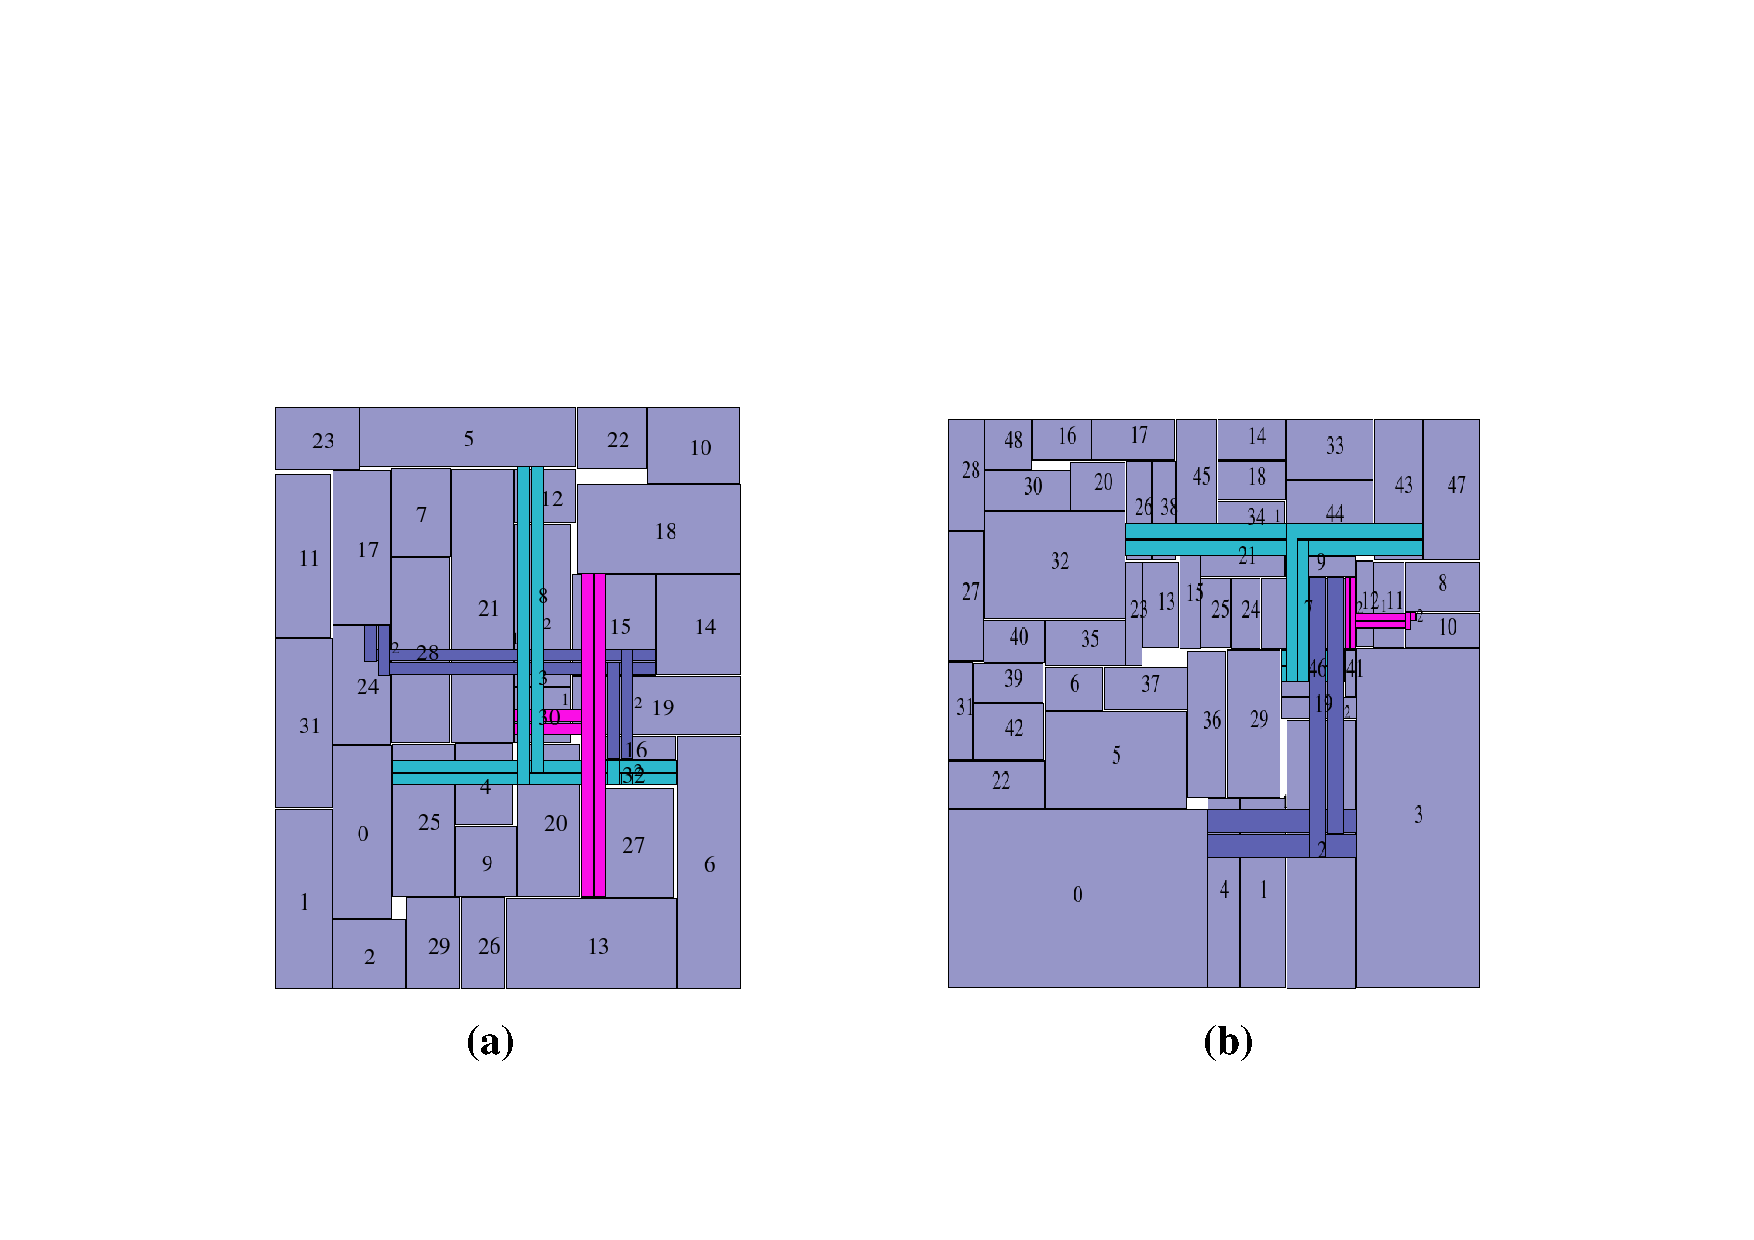
\includegraphics[width=11cm]{Fig/packing_result1.pdf}}
  %\centerline{\psfig{figure=Fig/packing_result1.eps, width=11cm}}
     \caption{
      (a) Packing result of ami33-i. The buses are \{13, 16, 18, 19, 21, 27, 30\}, \{0, 5, 6, 20, 25, 30, 32\},
                                                   \{14, 15, 16, 17, 24, 28, 32\}.
      (b) Packing result of ami49-h. The buses are \{7, 8, 9, 10, 11, 12, 41\}, \{29, 32, 41, 43, 44, 46, 47\},
                                                   \{0, 1, 2, 3, 4, 9, 46\}.
   }
  \label{fig::packing_result1}
\end{figure}

\begin{figure*}[htb]
{
  \centering
  \scriptsize
   TABLE III: COMPARISON BETWEEN \cite{PH10} AND THIS WORK
    \centerline{\includegraphics[width=17cm]{Fig/table_3.pdf}}\\
    %\centerline{\psfig{figure=Fig/table_3.eps, width=17cm}}\\
    $^*$The deviation at each load is estimated by total number of turning nodes from the driver to the load divided by total number of loads.\\
    $^{**}$The deviation (D) is obtained by the algorithm which is published in GLSVLSI 2010.\\
    $^{***}$The deviation (D) is obtained by the algorithm which is developed in this work.\\
  \label{fig::table3}
}
\end{figure*}

\section{The Comparison Between \cite{PH10} and This Work}
\label{sec::THE COMPARISON BETWEEN GLSVLSI 2010 AND THIS WORK}
In the remaining experiments, we are implemented our bus-driven floorplanner in C
language on a 2-GHz Linux machine with 16GB memory.
Since the work which is published on GLSVLSI 2010 only performs
the algorithm described in Section~\ref{sec::Deviation Minimization with Lookup Table Method}
after the SA, the deviation of each testcase could not
be minimized effectively. In this paper, we develop another efficient
approach to determine the deviation of each module such that
it can be integrated into the simulated annealing process.
The comparison results are shown in Table III.
Since the effect of the deviation is considered in this work during SA,
i.e., the solution space is much more constrained.
The run time is longer than GLSVLSI 2010 and the deadspace and wirelength are increased, however,
the deviation for each testcase can be further optimized to 0 as shown in the experimental results.

\section{The Comparison Between Modified \cite{PH10} and This Work}
\label{sec::The Comparison Between Modified GLSVLSI 2010 and This Work}
In this section, we modify the algorithm which is published in GLSVLSI 2010
such that it has the same structure with this work, i.e., the effect of
deviation is considered during SA.
The difference between the modified algorithm and this work is that
the algorithm described in Section ~\ref{sec::Deviation Minimization with Lookup Table Method}
is performed to determine the orientation of each bus pin in the modified algorithm, and
the algorithm described in ~\ref{sec::Fast Deviation Update Based on Topology Comparison}
is performed to determine the orientation of each bus pin in this work.
The comparison results are shown in Table IV.
The results show that deadspace, wirelength, success rate, and deviation is
nearly the same, nevertheless, the algorithm proposed in this paper is
run faster than the modified method.
Therefore, the proposed approach is more suitable on optimizing the
deviation during the SA.

\begin{figure*}[htb]
{
  \centering
  \scriptsize
   TABLE IV: COMPARISON BETWEEN MODIFIED \cite{PH10} AND THIS WORK
    \centerline{\includegraphics[width=17cm]{Fig/table_4.pdf}}\\
    %\centerline{\psfig{figure=Fig/table_4.eps, width=17cm}}\\
  \label{fig::table4}
}
\end{figure*}


\section{Experiments on Larger Testcases for \cite{PH10} and This Work}
\label{sec::EXPERIMENTS ON LARGER TESTCASES}

In this section, we will perform the experiments on larger testcases for the algorithm which is
published in GLSVLSI 2010 and this work.
The set of testcases are derived from n100, n200, n300 with bus sizes ranging from 10 to 40.
The details of all testcases are listed in Table V.
\begin{figure}[htb]
{
  \centering
  \scriptsize
   TABLE V: LARGER TESTCASE STATISTICS\\
   \centerline{\includegraphics[width=10cm]{Fig/table_5.pdf}}
   %\centerline{\psfig{figure=Fig/table_5.eps, width=10cm}}

  \label{fig::table5}
}
\end{figure}

\begin{figure*}[htb]
{
  \centering
  \scriptsize
   TABLE VI: COMPARISON BETWEEN \cite{PH10} AND THIS WORK ON LARGER TESTCASES
   \centerline{\includegraphics[width=17cm]{Fig/table_6.pdf}}\\
    %\centerline{\psfig{figure=Fig/table_6.eps, width=17cm}}\\
  \label{fig::table6}
}
\end{figure*}

To the best of our knowledge, no previous works can handle the buses with
such a large net size.
The comparison results are shown in Table VI.
The experimental results show that our algorithm performs better in success rate by 1.03$\times$,
deviation by 16.64$\times$, and reduces the deadspace 1.11$\times$.
Since it has to minimize the deviation during SA, it constrains the solution
space such that the bus wirelength are increased and spends more time on adjusting
the bus shape to obtain a better solution. However, the deviation can be further optimized to 0 in lots of
the testcases, and the deviation is effectively minimized in the difficult testcases.
Some packing results are shown in Figure~\ref{fig::packing_result2}.

\begin{figure}[htb]
  \centering
  \centerline{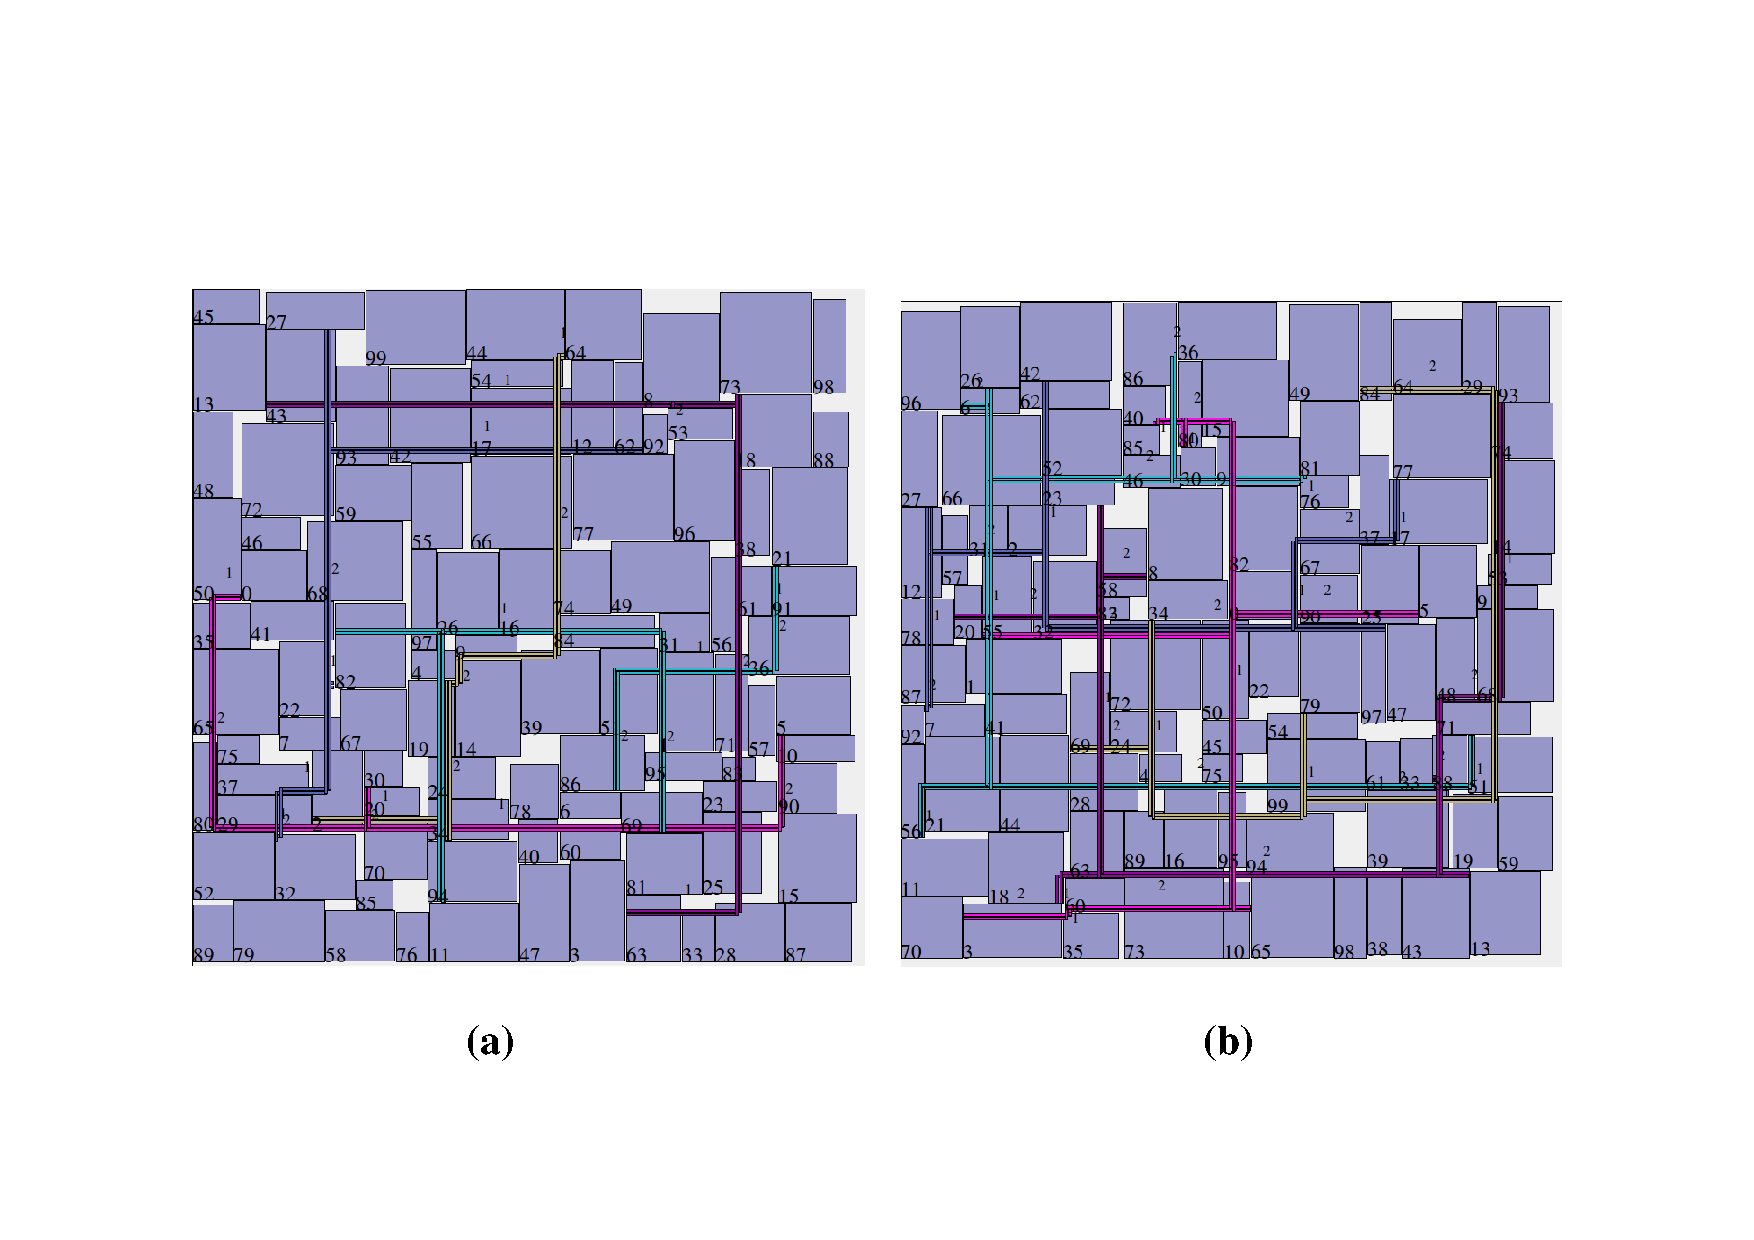
\includegraphics[width=13cm]{Fig/packing_result2.pdf}}
  %\centerline{\psfig{figure=Fig/packing_result2.eps, width=13cm}}
     \caption{
      (a) Packing result of n100-c. The buses are \{0, 10, 20, 30, 40, 50, 60, 70, 80, 90, 5, 15, 25, 35\},
                                                  \{1, 11, 21, 31, 41, 51, 61, 71, 81, 91, 6, 16, 26, 36\},
                                                  \{2, 12, 22, 32, 42, 52, 62, 72, 82, 92, 7, 17, 27, 37\},
                                                  \{3, 13, 23, 33, 43, 53, 63, 73, 83, 93, 8, 18, 28, 38\},
                                                  \{4, 14, 24, 34, 44, 54, 64, 74, 84, 94, 9, 19, 29, 39\}.
      (b) Packing result of n100-f. The buses are \{0, 10, 20, 30, 40, 50, 60, 70, 80, 90, 5, 15, 25, 35, 45, 55, 65, 75, 85, 95\},
                                                  \{1, 11, 21, 31, 41, 51, 61, 71, 81, 91, 6, 16, 26, 36, 46, 56, 66, 76, 86, 96\},
                                                  \{2, 12, 22, 32, 42, 52, 62, 72, 82, 92, 7, 17, 27, 37, 47, 57, 67, 77, 87, 97\},
                                                  \{3, 13, 23, 33, 43, 53, 63, 73, 83, 93, 8, 18, 28, 38, 48, 58, 68, 78, 88, 98\},
                                                  \{4, 14, 24, 34, 44, 54, 64, 74, 84, 94, 9, 19, 29, 39, 49, 59, 69, 79, 89, 99\}.
   }
  \label{fig::packing_result2}
\end{figure}

